\section{Desarrollo}
	Se realizó una simulación del juego de la vida, con un tamaño de población de 100x100, en la figura \ref{fig:patron1} se muestra una gráfica del total de organismos vivos (unos), entre el número de generación. Se muestra que además el promedio y la densidad. La cual resultó ser continua en un valor de 0.4010

	\begin{figure}[H]
		\begin{center}
			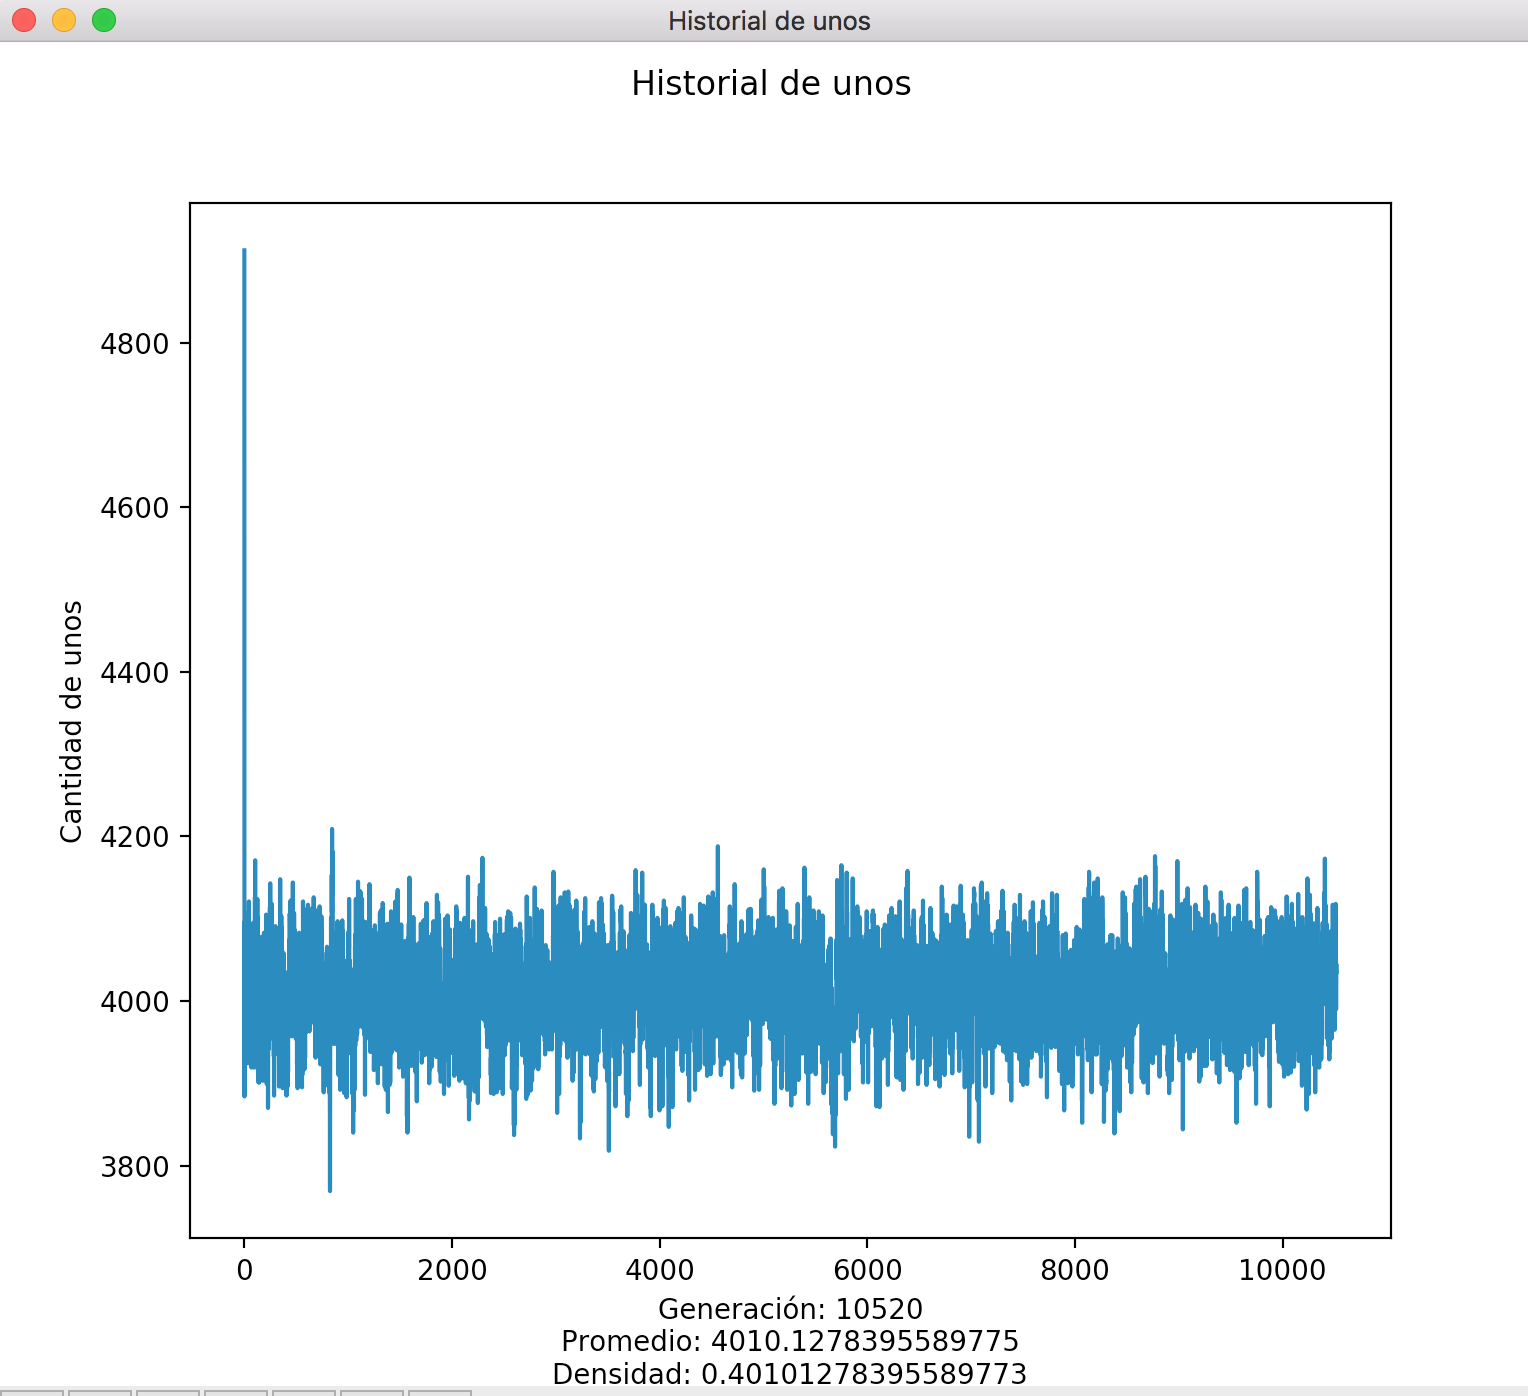
\includegraphics[scale=.5]{img/grafica.png}
			\caption{Gráfica de total de unos, que muestra promedio y densidad}
			\label{fig:patron1}
		\end{center}
	\end{figure}

	% \begin{figure}[H]
	% 	\begin{center}
	% 		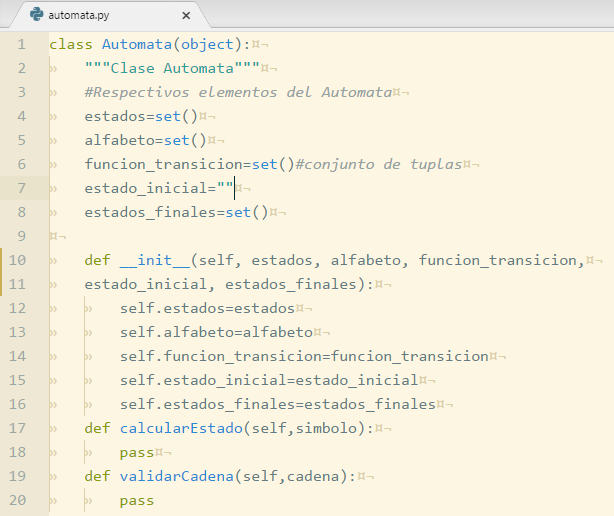
\includegraphics[width=15cm, height=12cm]{img/automata.png}
	% 		\caption{automata.py}
	% 		\label{fig:tablas}
	% 	\end{center}
	% \end{figure}